\subsection{Data flow}
\subsubsection{Overview}There are a lot of cases when we want to make several actions in response of one HTTP request. Moreover, subset of those actions is the same for more than one function and the requirement to proceed to next step (fire next action) is the successful return from the current one. To achieve that dataflow mechanism has been created.

The basic idea is to provide a tool for defining flow of data from beginning
of the request to its end. For example, we can specify, that before calling
{\bf user:create} we want to check the permissions of the caller, validate
input data, check for uniqueness, log the activity and only if every of them
has ended successfully - proceed to {\bf create} function. It is possible also
to declare some functions to execute after fuction requested by HTTP server
(syntax in the next paragraph). In that case we do not have to worry about
arguments requested by HTTP server mode -- it is captured and values passed by
"after request" functions are up to developer's idea. 

\subsubsection{Control flow}To enable the mechanism of dataflow, controller module, which we want to use dataflow within, must export {\bf dataflow/1} and {\bf error/2} functions. 
\paragraph{dataflow/1}- Function {\bf dataflow/1} is responsible for providing the list of functions inside its module, which will be sequentially called, one after another. Each of that function must return either {\it \{ok, }{\bf {\em Args}}{\it \}} or {\it \{error, }{\bf {\em Reason}}{\it \}} tuple. \newline
Specification:
\begin{Verbatim}
dataflow(ControllerFun) -> {BeforeList, AfterList} | BeforeList

BeforeList = AfterList = [Function]
ControllerFun = Function = atom()
\end{Verbatim}

{\bf Args} will be used as the arguments for the next function in dataflow list or as the arguments for the proper function call. 

The proper function will be called only when all the functions specified in {\bf dataflow} will succeed (and it will be called with arguments returned from the last function on the dataflow's list). 
\paragraph{error/2}- If something goes wrong and one of the functions will return an error, the calling sequence is stopped and the {\bf error(FunName, Reason)} is called ({\bf FunName} is the name of the function where error occured)

If one of the obligatory dataflow functions is not present (exported), the standard procedure is held: at first the {\bf validate/1} function is called, then the proper one is fired.
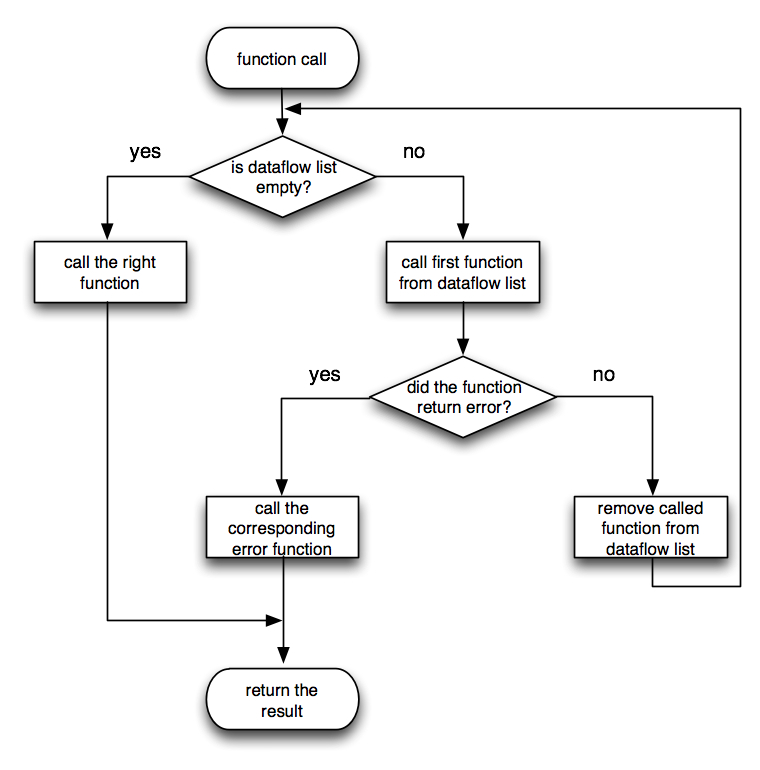
\includegraphics[width=\textwidth]{images/dataflow.jpg}

\subsubsection{Example}Let's assume we want to create the following scenario of removing user from system \\({\bf users:remove/1} function - argument is an ID of the user):
\begin{enumerate}
\item check if user connects {\it via} https
\item check if user has right permissions
\item validate passed parameters (passed in URL, like: {\it users/delete/3} to remove user with ID=3)
\item log the activity
\item proceed the removal function
\end{enumerate}
To achieve this {\bf users} module must at least look like that:
\begin{Verbatim}[numbers=left]
...
-export([dataflow/1, error/2]).
...
dataflow(remove) -> [check_https, check_permissions, 
                     validate_number, log].
...
check_https(_, _) ->
  case wpart:fget("__https") of
    true  -> {ok, ok};
    false -> {error, no_https}
  end.

check_permissions(_, ok) ->
  %% check if user is logged in and has the good permissions
  case Result of
    not_logged_in             -> {error, not_logged_in};
    not_enough_permissions    -> {error, not_enough_permissions};
    _                         -> {ok, ok}
  end.

validate_number(_, ok) ->
  case validate_tool:validate_number() of
    {error, default_val} -> {ok, 1};
    {error, nan}         -> {error, invalid_url};
    {ok, N}              -> {ok, N}
  end.

log(Action, Number) ->
  %% log activity to the file
  {ok, Number}.

error(check_https, no_https) ->
  {redirect, "https://" ++ e_conf:host() ++ wpart:fget("__path")};
error(check_permissions, not_logged_in) ->
  {redirect, "/login"};
error(check_permissions, not_enough_permissions) ->
  {template, "/errors/not_enough_permissions.html"};
error(validate_number, invalid_url) ->
  {error, 404}.

remove(Number) ->
  %% proceed with user removal
  {template, "users/list.html"}.

...
\end{Verbatim}
